%%%%%%%%%%%%%%%%%%%%%%%%%%%%%%%%%%%%%%%%%%%%%%%%%%%%%%%%%%%%%%%%%%%%%%%%%%%%%%%%
%2345678901234567890123456789012345678901234567890123456789012345678901234567890
%        1         2         3         4         5         6         7         8

\documentclass[a4, 10 pt, conference]{ieeeconf}  % Comment this line out if you need a4paper

%\documentclass[a4paper, 10pt, conference]{ieeeconf}      % Use this line for a4 paper

\IEEEoverridecommandlockouts                              % This command is only needed if 
                                                          % you want to use the \thanks command

\overrideIEEEmargins                                      % Needed to meet printer requirements.

% See the \addtolength command later in the file to balance the column lengths
% on the last page of the document

% The following packages can be found on http:\\www.ctan.org
%\usepackage{graphics} % for pdf, bitmapped graphics files
%\usepackage{epsfig} % for postscript graphics files
%\usepackage{mathptmx} % assumes new font selection scheme installed
%\usepackage{times} % assumes new font selection scheme installed
%\usepackage{amssymb}  % assumes amsmath package installed
\usepackage{multicol}
\usepackage{tcolorbox}
\usepackage{cuted,tcolorbox,lipsum}
\usepackage{xcolor}
\usepackage{amsmath}
\usepackage{float}

\title{\LARGE \bf
Introduction to Machine Learning (SS 2025)\\ Programming Project
\vspace{-3em}
}


%\author{Someone Anyone$^{1}$ and Xiang Zhang$^{2}$% <-this % stops a space
%}


\begin{document}


\maketitle
\vspace{-3em}
\thispagestyle{empty}
\pagestyle{empty}

\begin{strip}
  \begin{tcolorbox}[
      size=tight,
      colback=white,
      boxrule=0.2mm,
      left=3mm,right=3mm, top=0mm, bottom=0mm
    ]
    {\begin{multicols}{3}% replace 3 with 2 for 2 authors.

        \textbf{Author 1}       \\
        Last name:    Schweigl    \\  % Enter first name
        First name:   Dominik    \\  % Enter first name
        Matrikel Nr.: 12243381              \\  % Enter Matrikel number

        \columnbreak

        \textbf{Author 2}       \\
        Last name:    Schöpf          \\  % Enter first name
        First name:   Emanuel          \\  % Enter first name
        Matrikel Nr.:               \\  % Enter Matrikel number

        \columnbreak

        % only four three person team
        % \textbf{Author 3}       \\
        % Last name:              \\  % Enter first name
        % First name:             \\  % Enter first name
        % Matrikel Nr.:               \\  % Enter Matrikel number

      \end{multicols}}
  \end{tcolorbox}
\end{strip}

%%%%%%%%%%%%%%%%%%%%%%%%%%%%%%%%%%%%%%%%%%%%%%%%%%%%%%%%%%%%%%%%%%%%%%%%%%%%%%%%

\section{Introduction}
\label{sec:intro}

For this report the task consists of classifying images of sign language hand gestures.
The dataset contains a total of 9680 instances of hands in a 128 x 128 pixel grayscale format.
Hence, this is a multilabel classification task, where each image corresponds to a
sign of the digits 0 to 9 and the letters a to z, totaling 36 classes.

The dataset is considerably imbalanced with the frequency for each sign ranging from
1.07\% to 5.78\%. 9 of the classes have frequencey of 5.78\%, 6 classes have
frequency of 2.89\%, and the rest has ~1.50\% frequency.

\section{Implementation / ML Process}
\label{sec:methods}

The methods chosen for this task are a convolutional neural network (CNN), as
well as a multilabel support-vector-machine (SVM) classifier.

\subsection{Data preprocessing}
\label{subsec:preprocessing}

In order to avoid the machine learning methods not account well for minority classes or
learning wrong sign distributions or ignore minority classes and always predict the majority class
and misleading metrics like 90\% overall precision but 0\% recall for minority classes,
the dataset was balanced by augmenting the instances of the minority classes.
The data was augmented using horizontal mirroring as well as 90\textdegree/$-90$\textdegree rotation based
on how much augmentation was needed per class. The result is a dataset consisting
of 18056 instances with frequencies in the range of 2.48\% to 3.10\%.

For the CNN it was found that more data was needed to increase the accuracy of the model
above 87\%. Therefore a dynamic data loader was implemented, which increases the
dataset size by a specified factor using random augmentation of 15\textdegree rotation,
horizontal mirroring, and random scaling between 80\% to 100\%. For the following
a factor of 2 was used resulting in a dataset of 36112 instances with unchanged frequencies.

For the SVM classifier it was found necessary to scale the image values by $\frac{1}{255}$
to obtain features in the range $[0,1]$ for numerical stability. Furthermore, it was found that it is not feasible for SVMs to work with high dimensional inputs
like our image dataset. Hence, PCA preprocessing with 200 components was applied to the images for the
SVM classifier in order to retain 90\% explained variance.

\subsection{Classifier architecture}
\label{subsec:architecture}

A convolutional neural network (CNN) was chosen for this task due to its effectiveness in processing image data. CNNs use local receptive fields to focus on small image regions, capturing spatial patterns and relationships more effectively than fully connected networks.

The architecture begins with convolutional layers that apply small filters (kernels) to detect local patterns such as edges and textures. As training progresses, these kernels learn to extract features relevant to the classification task. Pooling layers reduce the spatial dimensions of feature maps, lowering computational cost and making the model more robust to translations. Max pooling, which selects the maximum value in each region, is commonly used.

At the end, fully connected layers aggregate the high-level features and map them to output classes. The chosen CNN consists of three convolutional layers (each followed by 2×2 max pooling) and two fully connected layers. This structure enables the model to learn hierarchical features from the 128×128 input and classify them into 36 categories.

The support vector machine (SVM), implemented via sklearn.svm.SVC, was chosen for its ability to maximize the soft margin between classes, offering robustness to outliers and irrelevant features—particularly useful with high-dimensional, PCA-transformed image data. SVMs generalize better than logistic regression when classes aren't linearly separable, thanks to kernel functions like linear, polynomial, and RBF, which enable non-linear decision boundaries via the kernel trick.

SVMs separate classes by finding the hyperplane that maximizes the margin defined by the nearest data points (support vectors). Multi-class classification is handled using one-vs-rest or one-vs-one strategies, both supported by scikit-learn. For $K$ classes, one-vs-one creates $\frac{K*(K-1)}{2}$ binary classifiers, with predictions made via majority voting.

SVMs minimize hinge loss:

\[
  \mathcal{L}_{hinge} = \max(0, 1 - y \cdot f(\mathbf{x}))
\]
where $f(\mathbf{x}) = \mathbf{w}^\top \mathbf{x} + b$ and $y \in \{0, 1\}$. Compared to log-loss used in logistic regression, hinge loss penalizes misclassifications less aggressively, making SVMs more robust to outliers.

Another approch was using an Autoencoder, but this did not give any accuracy boosts and was just more complex, than the CNN network.

\subsection{Hyperparameters}
\label{subsec:hyperparameters}

The hyperparameter optimization was realized with random search. For each
hyperparameter a numerical interval $[a, b]$ or a discrete set of choices $\{c,d,e,...\}$
was defined. Across 60 trials per classifier hyperparameters are uniformly sampled according
to the defined bounds, which are used to train a model on the dataset. The model is
evaluated using validation set and the best set of hyperparameters is selected
based on the resulting models performance.
For The Hyperparameter optimization of the CNN classifier the maximum training epochs
were set to 10 and it was performed on the dataset without additional augmentation due
to time constraints.

For the CNN classifier, random search was performed with a maximum of 40 training epochs.
Early stopping was applied with a patience of 5 epochs, requiring a minimum improvement in
validation loss of 0.01. Additionally, if validation accuracy did not reach at least 40\% by
epoch 10, training was stopped early. The search optimized across batch size $B$, learning rate
$l_R$ sampled from log-scale to bias small learning rates, kernel size $k$, number of convolutional channels $C_c$, linear layer size $n_h$, dropout
rate $d$, and activation function $f_A$.

For the SVM classifier scikit-learns support vector classifier sklearn.svm.SVC was used.
The choice of the multi-class decision scheme OvO and OvR as well as the kernel function,
the regularization parameter $C$, the kernel coefficient $\gamma$, and for the
polynomial kernel the degree $d$ and the bias term $coef0$ were examined.

\section{Results}
\label{sec:results}

The CNN classifier yiels significantly better results than the SVM classifier.
The final accuracies are shown in Table~\ref{tab:classifier_accuracy}.


\begin{table}[H]
  \centering
  \begin{tabular}{|l|c|c|c|}
    \hline
        & Train set & Validation set & Test set \\
    \hline
    CNN & 98.89\%   & 98.56\%        & 96.25\%  \\
    SVM & 97.76\%   & 87.62\%        & 85.21\%  \\
    \hline
  \end{tabular}
  \caption{Final classifier accuracy on training, validation, and testing.}
  \label{tab:classifier_accuracy}
\end{table}

\vspace{-1.5em}

The majority of remaining inaccuracy for both classifiers stem from a small set of similar
looking sign pairs, namely (O,0), (V,2), (W,6), and (M,N). This is clearly visible
in their respective confusion matrices shown in Figure~\ref{fig:cm}. The SVM
classifier shows small amounts of confusion across the whole set of classes,
which explains the significantly lower validation accuracy.

\begin{figure}[htb]
  \centering
  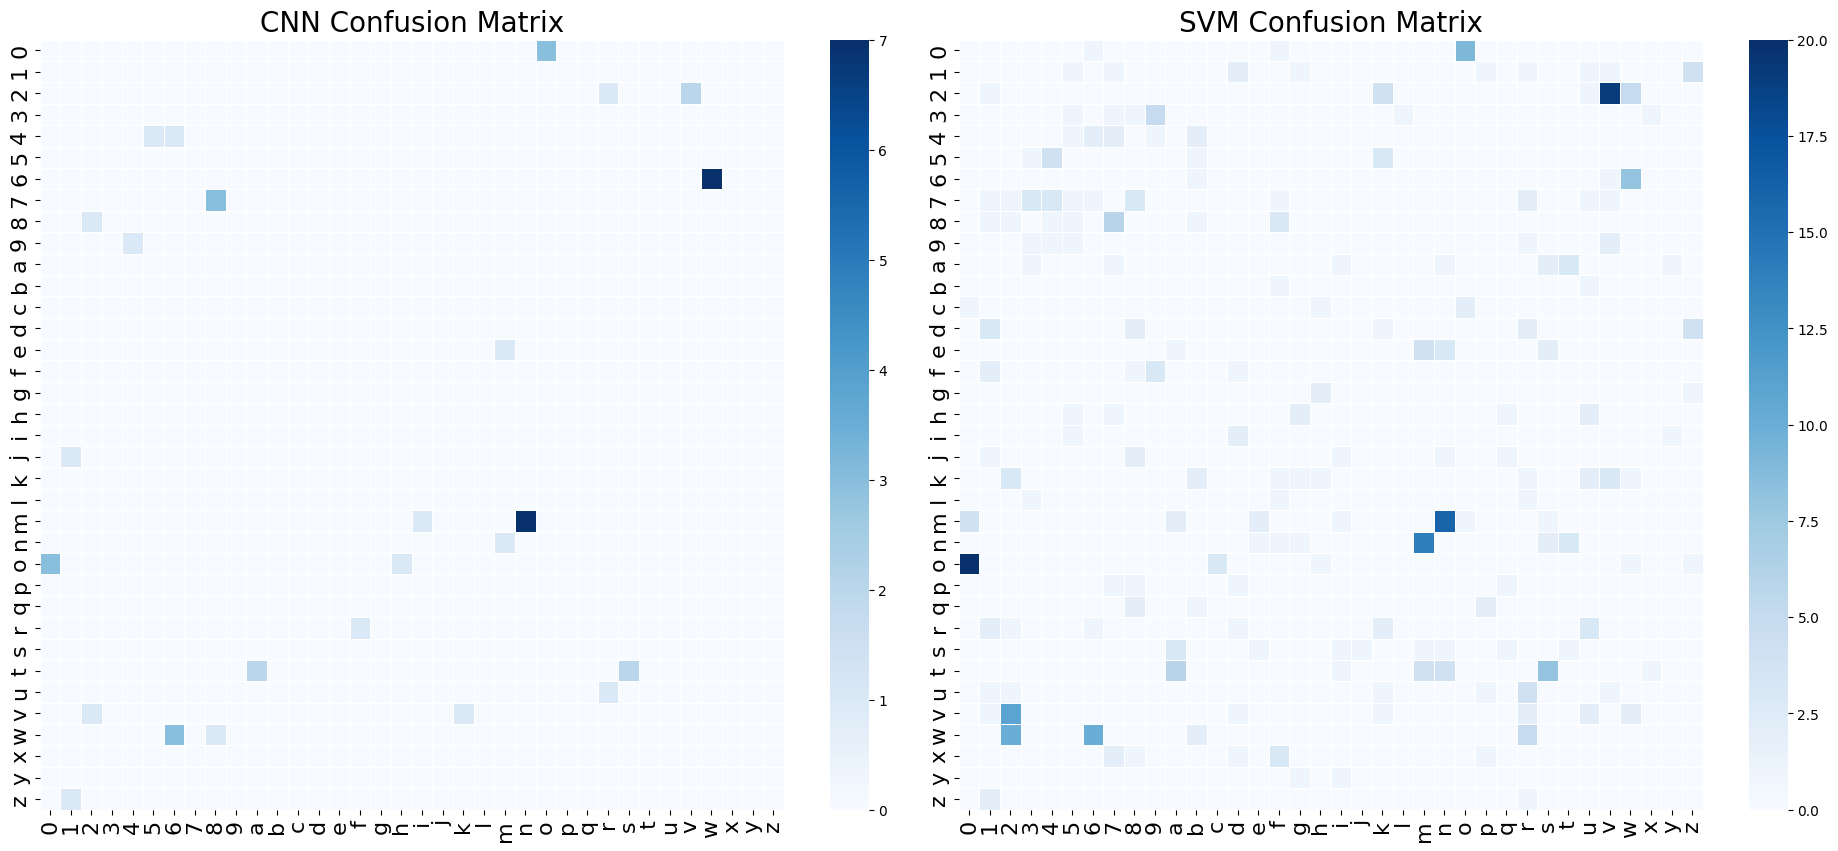
\includegraphics[width=\linewidth]{../images/cm_comparison.png}
  \caption{Confusion matrices for CNN and SVM classifiers with ommitted diagonal, predicted value (left) and actual value (bottom).}
  \label{fig:cm}
\end{figure}

When plotting the per-class precision and accuracy values for the CNN classifier,
the pair wise confusion is seen by the duality between precision and recall of the
respective confused pairs.

\section{Discussion}
\label{sec:discuss}

Initial attempts to train the SVM on raw 128x128 image inputs without normalization or feature extraction failed to converge, highlighting SVMs' poor scalability to high-dimensional data. After applying PCA for dimensionality reduction, performance improved significantly. However, the final model size exceeded the 50 MB limit—reaching around 60 MB (50 MB for the SVM, 10 MB for PCA)—despite optimizations like switching from an RBF to a polynomial kernel, using One-vs-Rest, and reducing PCA components from 500 to 200. Surprisingly, these changes did not hurt performance.

Further size reduction to 37 MB was achieved by removing extra data augmentation and reverting to a balanced dataset, which reduced the number of support vectors, at the cost of ~1\% accuracy loss. Replacing PCA with an autoencoder could yield more compact, informative features for the SVM.

For the CNN classifier, performance gains were primarily driven by dataset expansion and targeted augmentation, particularly for underrepresented classes. Early models failed to classify class W entirely until class balancing was introduced. A deeper CNN with smaller kernels could further improve accuracy by capturing finer details, but was not explored due to the 50 MB model size limit—the current CNN already used 49 MB.


\section{Conclusion}
\label{sec:con}

The final CNN classifier was trained for 60 epochs on the entire training
dataset and achieved a strong test dataset accuracy of 96.25\%. In comparison,
the SVM classifier reached a respectable y\%. While SVMs can be a viable
alternative to CNNs for small multi-label classification tasks -- especially
those involving few classes, small image sizes, and moderate amounts of
data such as the MNIST dataset -- they do not scale as effectively as CNNs
to big data sets with large images and many classes. This limitation persists even after
dimensionality reduction with PCA, whereas learning compact representations
with a convolutional autoencoder may provide feature spaces in which SVMs remain competitive.


%%%%%%%%%%%%%%%%%%%%%%%%%%%%%%%%%%%%%%%%%%%%%%%%%%%%%%%%%%%%%%%%%%%%%%%%%%%%%%%%



\end{document}
